% hitex-deck-style: 2
\documentclass[aspectratio=169,11pt]{beamer}
\graphicspath{{../}}
\usetheme{default}
\usepackage{graphicx}
\usepackage{amsmath}
\usepackage{amssymb}
\usepackage{booktabs}
\usepackage{tikz}
\definecolor{hxStructure}{HTML}{00695C}
\definecolor{hxAccent}{HTML}{C2185B}
\definecolor{hxMuted}{HTML}{5F6B69}
\definecolor{hxText}{HTML}{1F2328}
\definecolor{hxBackground}{HTML}{FFFFFF}
\definecolor{hxTitleBg}{HTML}{F1F8F7}
\definecolor{hxTitleFg}{HTML}{00695C}
\definecolor{hxRule}{HTML}{BFDAD6}
\definecolor{hxTint}{HTML}{94C0BB}
\setbeamercolor{normal text}{fg=hxText,bg=hxBackground}
\setbeamercolor{background canvas}{bg=hxBackground}
\setbeamercolor{structure}{fg=hxStructure}
\setbeamercolor{title}{fg=hxStructure}
\setbeamercolor{frametitle}{fg=hxStructure}
\setbeamercolor{subtitle}{fg=hxMuted}
\setbeamercolor{author}{fg=hxText}
\setbeamercolor{alerted text}{fg=hxAccent}
\setbeamercolor{page number in head/foot}{fg=hxMuted}
\setbeamercolor{itemize item}{fg=hxStructure}
\setbeamercolor{itemize subitem}{fg=hxMuted}
\setbeamerfont{title}{series=\bfseries}
\setbeamerfont{frametitle}{series=\bfseries}
\setbeamertemplate{navigation symbols}{}
\setbeamertemplate{itemize item}{\raisebox{0.12em}{\rule{0.4em}{0.4em}}}
\setbeamertemplate{itemize subitem}{\textendash}
\makeatletter
\newcommand{\hxframes}{11}
% n / N: the total from the last run, or this deck's own count before there is one
\newcommand{\hxtotal}{\ifnum\inserttotalframenumber<\insertframenumber\relax\hxframes\else\inserttotalframenumber\fi}
\setbeamertemplate{frametitle}{%
  \vskip0.45cm%
  \begin{beamercolorbox}[wd=\paperwidth,leftskip=1cm,rightskip=1cm plus 1fil,sep=0pt]{frametitle}%
    \usebeamerfont{frametitle}\insertframetitle\par
    \ifx\insertframesubtitle\@empty\else{\small\color{hxMuted}\insertframesubtitle\par}\fi
    \nointerlineskip\vskip5pt{\color{hxAccent}\rule{1.2cm}{2.5pt}}\par
  \end{beamercolorbox}}
\setbeamertemplate{footline}{%
  \hbox to \paperwidth{\hskip1cm{\color{hxRule}\rule{\dimexpr\paperwidth-2cm\relax}{0.4pt}}\hss}%
  \vskip3pt%
  \hbox to \paperwidth{\hskip1cm\usebeamerfont{page number in head/foot}\usebeamercolor[fg]{page number in head/foot}%
    \insertshorttitle\hfill\insertframenumber\,/\,\hxtotal\hskip1cm}%
  \vskip6pt}
% Title, section and closing slides: a plain frame whose page background is drawn once by \hx@bg.
\let\hx@bg\@empty
\setbeamertemplate{background}{\ifx\hx@bg\@empty\else\hx@bg\global\let\hx@bg\@empty\fi}
% The title and closing slides: the title art (title-art.jpg, next to this file) full-bleed, its left
% side already the title background, and the text set on it on the left.
\newcommand*{\hxpresenter}{}
\newcommand*{\hxcoauthors}{}
\newcommand{\hx@art}[1]{%
  \IfFileExists{title-art.jpg}%
    {\node[anchor=south west,inner sep=0] at (0,0) {
\includegraphics[width=\paperwidth,height=\paperheight]{title-art.jpg}};}%
    {\fill[hxTitleBg] (0,0) rectangle (\paperwidth,\paperheight);}%
  \ifnum#1=1 \fill[hxTitleBg,opacity=0.3] (0,0) rectangle (\paperwidth,\paperheight);\fi}
% Fitting: the title block hangs from 1.2 cm below the top, the author block stands on 0.9 cm above the
% bottom, with at least 0.6 cm (and the accent rule) between them. Measured in saveboxes in one pass;
% when they do not fit: affiliations \tiny, then co-authors \footnotesize, then the title block scaled
% (down to 60 %), then the whole stack scaled.
\newsavebox\hx@titlebox
\newsavebox\hx@authbox
\newdimen\hx@colw
\newdimen\hx@avail
\newdimen\hx@th
\newdimen\hx@ah
\newcommand{\hx@nohyph}{\hyphenpenalty=10000\exhyphenpenalty=10000\raggedright}
\newcommand{\hx@buildtitle}[2]{% #1 title, #2 subtitle (may be empty)
  \sbox\hx@titlebox{\parbox[t]{\hx@colw}{\hx@nohyph
    {\color{hxTitleFg}\huge\bfseries #1\par}%
    \ifx#2\@empty\else\vskip6pt{\color{hxText}\large\bfseries #2\par}\fi}}%
  \hx@th=\ht\hx@titlebox \advance\hx@th by \dp\hx@titlebox}
\newcommand{\hx@buildauthors}[2]{% #1 co-author size, #2 affiliation size
  \sbox\hx@authbox{\parbox[b]{\hx@colw}{\hx@nohyph\color{hxText}%
    {\bfseries\hxpresenter\par}%
    \ifx\hxcoauthors\@empty\else\vskip2pt{#1\hxcoauthors\par}\fi
    \ifx\insertinstitute\@empty\else\vskip4pt{#2\color{hxMuted}\insertinstitute\par}\fi}}%
  \hx@ah=\ht\hx@authbox \advance\hx@ah by \dp\hx@authbox}
\newcommand{\hx@fits}{\dimexpr\hx@th+\hx@ah\relax<\hx@avail}
\newcommand{\hxtitleslide}{\gdef\hx@bg{%
  \hx@colw=0.6\paperwidth
  \hx@avail=\paperheight \advance\hx@avail by -2.7cm \advance\hx@avail by -8.5pt
  \hx@buildtitle{\inserttitle}{\insertsubtitle}%
  \hx@buildauthors{\small}{\scriptsize}%
  \ifdim\hx@fits\else\hx@buildauthors{\small}{\tiny}\fi
  \ifdim\hx@fits\else\hx@buildauthors{\footnotesize}{\tiny}\fi
  \gdef\hx@ts{1}\gdef\hx@as{1}%
  \ifdim\hx@fits\else
    \pgfmathsetmacro\hx@ts{max(0.6,(\hx@avail-\hx@ah)/max(\hx@th,1pt))}%
    \pgfmathparse{(\hx@ts*\hx@th+\hx@ah) > \hx@avail ? 1 : 0}%
    \ifnum\pgfmathresult>0
      \pgfmathsetmacro\hx@as{\hx@avail/(0.6*\hx@th+\hx@ah)}%
      \pgfmathsetmacro\hx@ts{0.6*\hx@as}%
    \fi
  \fi
  \begin{tikzpicture}
  \useasboundingbox (0,0) rectangle (\paperwidth,\paperheight);
  \hx@art{0}
  \node[anchor=north west,inner sep=0] at (1cm,\paperheight-1.2cm) {\scalebox{\hx@ts}{\usebox\hx@titlebox}};
  \node[anchor=south west,inner sep=0] (hxauthors) at (1cm,0.9cm) {\scalebox{\hx@as}{\usebox\hx@authbox}};
  \fill[hxAccent] ([yshift=7pt]hxauthors.north west) rectangle +(1.2cm,1.5pt);
  \end{tikzpicture}}}
\newcommand{\hxclosingslide}[2]{\gdef\hx@bg{%
  \hx@colw=0.6\paperwidth
  \hx@avail=\paperheight \advance\hx@avail by -2.1cm
  \sbox\hx@titlebox{\parbox[t]{\hx@colw}{\hx@nohyph
    {\color{hxTitleFg}\huge\bfseries #1\par}\vskip9pt{\color{hxAccent}\rule{1.2cm}{1.5pt}}\par\vskip6pt
    {\color{hxText}\large #2\par}}}%
  \hx@th=\ht\hx@titlebox \advance\hx@th by \dp\hx@titlebox
  \gdef\hx@ts{1}%
  \ifdim\hx@th>\hx@avail \pgfmathsetmacro\hx@ts{\hx@avail/\hx@th}\fi
  \begin{tikzpicture}
  \useasboundingbox (0,0) rectangle (\paperwidth,\paperheight);
  \hx@art{1}
  % the block's top at 24 % of the height, raised (to 1.2 cm) and then scaled when it is taller
  \pgfmathsetmacro\hx@top{min(0.24*\paperheight, max(1.2cm, \paperheight-0.9cm-\hx@ts*\hx@th))}%
  \node[anchor=north west,inner sep=0] at (1cm,\paperheight-\hx@top pt) {\scalebox{\hx@ts}{\usebox\hx@titlebox}};
  \end{tikzpicture}}}
\newcommand{\hxsectionslide}[2]{\gdef\hx@bg{%
  \begin{tikzpicture}
  \useasboundingbox (0,0) rectangle (\paperwidth,\paperheight);
  \fill[hxStructure] (0,0) rectangle (0.3cm,\paperheight);
  \node[anchor=south west,inner sep=0,text=hxTint] at (1.6cm,0.5\paperheight+0.1cm)
    {\scalebox{2.2}{\Huge\bfseries #1}};
  \node[anchor=north west,inner sep=0,text width=\paperwidth-3.2cm,align=left,text=hxStructure]
    at (1.6cm,0.5\paperheight-0.25cm) {\hyphenpenalty=10000\exhyphenpenalty=10000\LARGE\bfseries #2\par};
  \end{tikzpicture}}}
\makeatother

\title[A Blockchain-Verified Ensemble xAI Framework for CCS...]{A Blockchain-Verified Ensemble xAI Framework for CCS Monitoring}
\subtitle{Predictive, explainable, and auditable carbon capture and storage monitoring}
\author{Ihunanya Udodiri Ajakwe, Victor Ikenna Kanu, Simeon Okechukwu Ajakwe, Dong-Seong Kim}
\institute{Kumoh National Institute of Technology, Gumi, South Korea\\Kyungdong University, Global Campus, South Korea}
\renewcommand*{\hxpresenter}{Ihunanya Udodiri Ajakwe}
\renewcommand*{\hxcoauthors}{Victor Ikenna Kanu, Simeon Okechukwu Ajakwe, Dong-Seong Kim}
\date{}

\begin{document}

\begin{frame}[plain]
\hxtitleslide
\end{frame}

\begin{frame}{Outline}
\large
\textcolor{hxAccent}{\textbf{01}}\hspace{0.8em}\textcolor{hxStructure}{Motivation}\par\medskip
\textcolor{hxAccent}{\textbf{02}}\hspace{0.8em}\textcolor{hxStructure}{Approach}\par\medskip
\textcolor{hxAccent}{\textbf{03}}\hspace{0.8em}\textcolor{hxStructure}{Evidence}\par\medskip
\end{frame}

\section{Motivation}
\begin{frame}[plain]
\hxsectionslide{01}{Motivation}
\end{frame}

\begin{frame}{Why CCS Monitoring Needs Trust}
\begin{itemize}
\setlength{\itemsep}{0.6em}
\item{} CCS deployment requires continuous monitoring across distributed infrastructures.
\item{} Existing AI solutions can remain opaque to stakeholders.
\item{} Distributed decisions need traceability, integrity, and verifiable communication.
\item{} Predictive analytics, explanations, and validation are rarely unified.
\end{itemize}
\note{CCS systems combine heterogeneous data, distributed infrastructure, and consequential operational decisions. Existing AI can provide predictions without clearly explaining them or preserving their provenance. This paper addresses that gap by combining prediction, explainability, and blockchain-based verification.}
\end{frame}

\begin{frame}{A Four-Layer Auditable Pipeline}
\begin{columns}[c]
\begin{column}{0.56\textwidth}
\centering
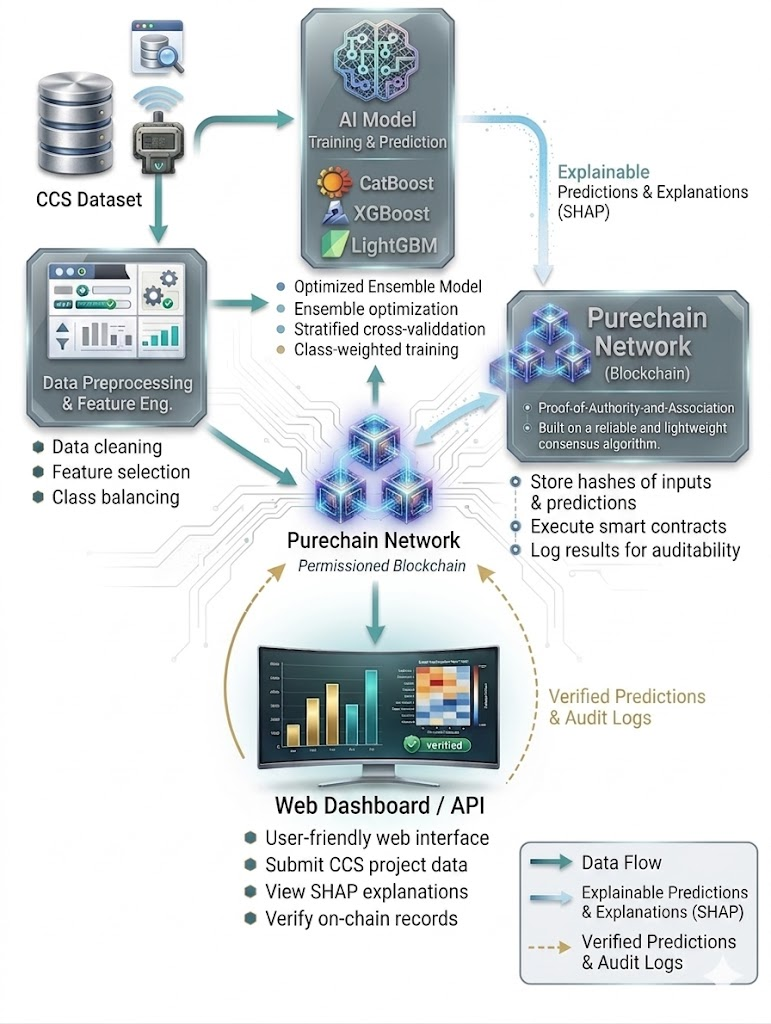
\includegraphics[width=\linewidth,height=0.78\textheight,keepaspectratio]{images/ICTC_system design3.jpeg}
\end{column}
\begin{column}{0.41\textwidth}
\small
\begin{itemize}
\setlength{\itemsep}{0.6em}
\item{} Data ingestion prepares heterogeneous project, technical, financial, and geographic attributes.
\item{} Ensemble prediction produces status; SHAP attributes feature contributions.
\item{} Purechain records outputs and explanations for stakeholder verification.
\end{itemize}
\end{column}
\end{columns}
\note{The proposed system connects four functions: data acquisition, intelligent modeling, blockchain verification, and user presentation. A project record is transformed into a status prediction and an explanation. The prediction and associated metadata are then recorded for later verification.}
\end{frame}

\section{Approach}
\begin{frame}[plain]
\hxsectionslide{02}{Approach}
\end{frame}

\begin{frame}{Stacked Ensemble and Explanation}
\begin{itemize}
\setlength{\itemsep}{0.6em}
\item{} CatBoost, XGBoost, and LightGBM serve as complementary base learners.
\item{} Logistic regression combines their probabilistic outputs.
\item{} Domain interactions include cost by technology and policy support.
\item{} Stratified validation, class weighting, and SMOTE address imbalance.
\item{} KernelExplainer provides global and local SHAP interpretations.
\end{itemize}
\note{The predictive core extends the CatBoost baseline into a stacked ensemble. The models receive engineered interactions intended to capture coupled financial, technological, and institutional effects. Stratification, weighting, and SMOTE address imbalance, while SHAP provides both global feature rankings and local explanations.}
\end{frame}

\section{Evidence}
\begin{frame}[plain]
\hxsectionslide{03}{Evidence}
\end{frame}

\begin{frame}{Performance Gains and Remaining Gap}
\begin{columns}[c]
\begin{column}{0.56\textwidth}
\centering
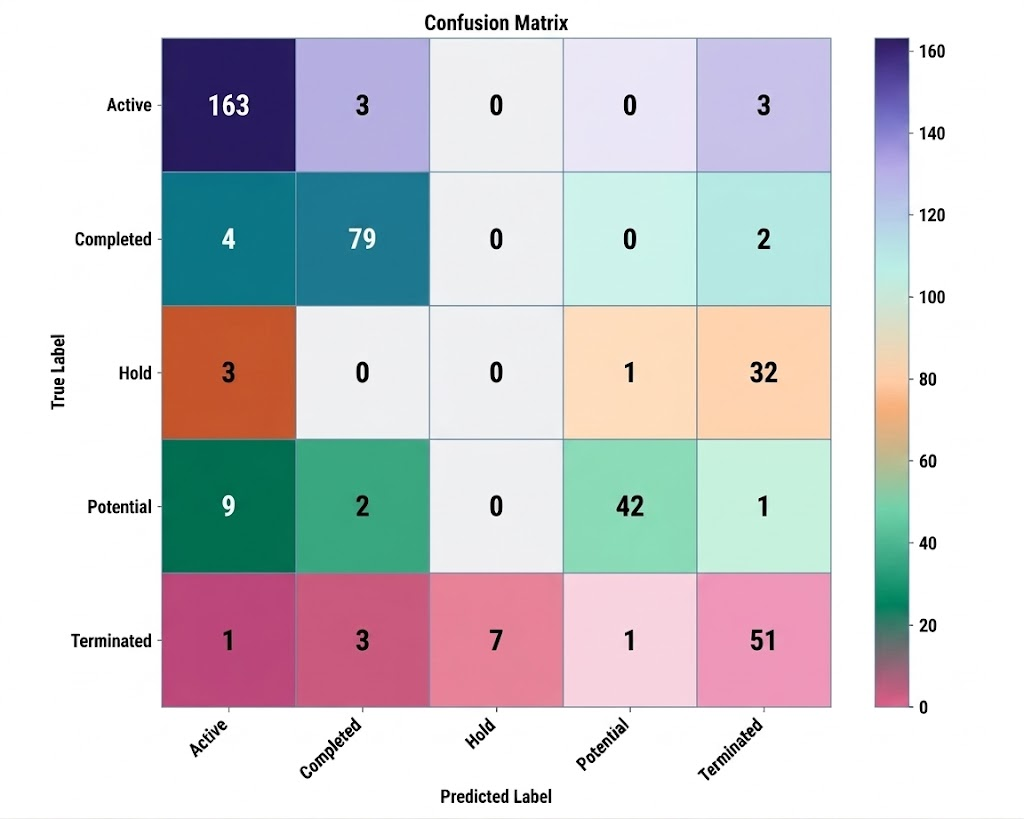
\includegraphics[width=\linewidth,height=0.78\textheight,keepaspectratio]{images/cm2.jpeg}
\end{column}
\begin{column}{0.41\textwidth}
\small
\begin{itemize}
\setlength{\itemsep}{0.6em}
\item{} Accuracy: approximately 0.82; weighted F1-score: approximately 0.80.
\item{} Macro-average F1-score: 0.68; one-versus-rest AUC: approximately 0.87.
\item{} Active and Completed F1-scores: 0.93 and 0.92; Hold: 0.00.
\end{itemize}
\end{column}
\end{columns}
\note{The enhanced ensemble reaches approximately 0.82 accuracy and 0.80 weighted F1-score. It performs particularly strongly for Active and Completed projects, while the Hold class remains unresolved. The confusion matrix shows that the main remaining difficulty concerns transitional project states.}
\end{frame}

\begin{frame}{From Prediction to Audit}
\begin{columns}[c]
\begin{column}{0.56\textwidth}
\centering
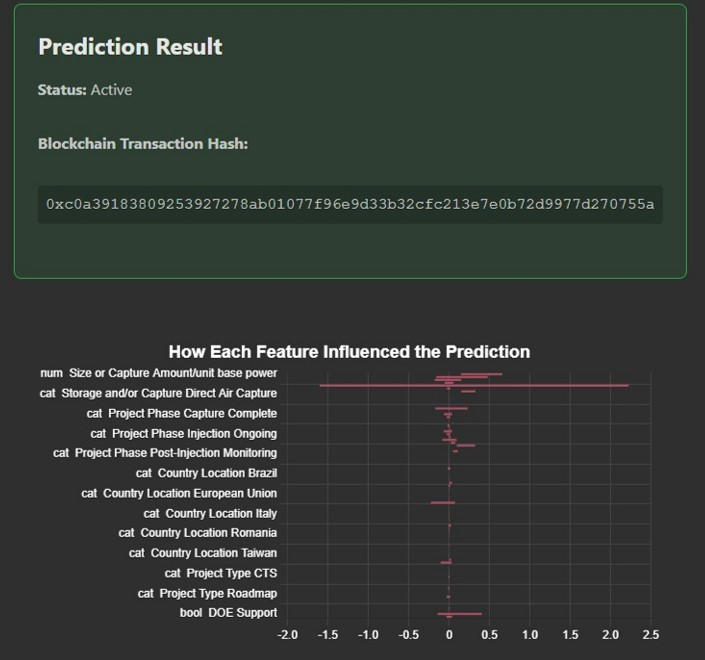
\includegraphics[width=\linewidth,height=0.78\textheight,keepaspectratio]{images/Prediction resulthash2.jpg}
\end{column}
\begin{column}{0.41\textwidth}
\small
\begin{itemize}
\setlength{\itemsep}{0.6em}
\item{} Purechain confirmation latency: 0.81 seconds; transaction cost: zero.
\item{} Verification success rate: 100 percent.
\item{} The interface links prediction, SHAP explanation, and transaction hash.
\item{} Current evaluation uses static historical records, not live IoT streams.
\end{itemize}
\end{column}
\end{columns}
\note{The deployed interface presents the prediction, its SHAP-based rationale, and the corresponding blockchain transaction hash. The reported Purechain evaluation achieved 0.81-second average latency, zero transaction cost, and 100 percent verification success. The current study uses static historical records, so live IoT ingestion and continuous updating remain future work.}
\end{frame}

\begin{frame}[plain]
\hxclosingslide{Thank you}{Questions?}
\end{frame}

\end{document}
